% LaTeX Template for Including FoggyTCP Performance Plots
% This template shows how to properly include the generated PDF plots in your LaTeX document

\documentclass[11pt,letterpaper]{article}
\usepackage[utf8]{inputenc}
\usepackage{graphicx}
\usepackage{float}
\usepackage{caption}
\usepackage{subcaption}
\usepackage{amsmath}
\usepackage{geometry}

% Set margins
\geometry{margin=1in}

\title{FoggyTCP Checkpoint 1 Report}
\author{CHOW Ho Sum Samson}
\date{\today}

\begin{document}

\maketitle

\section{Hypothesis}

In this checkpoint, we hypothesize that transmission time via a point to point 
network is modeled by the following equation:

\begin{equation}
    Time = \frac{File Size}{Bandwidth} + 2 \times Propagation Delay + Constant\_Overhead
\end{equation}

meaning that the transmission time is linearly proportional to the file size and propagation delay,
 and inversely proportional to the bandwidth.
  We expect that the experimental results will closely align with this theoretical model,
   with minor deviations due to various hardware overhead.


% We do know that TCP has some overhead, so we expect the experimental results to be slightly higher than the theoretical values.
%  However, we expect the overall trends to match closely, confirming the validity of our hypothesis.

\section{Experiment}    
\subsection{Setup}
The experiment was conducted using two virtual machines (VMs) connected via a point-to-point link.
 The server VM hosted the FoggyTCP server binary, while the client VM ran the client binary to send files.
  The network conditions were manipulated using traffic control (tconfig) to simulate different bandwidths and propagation delays.
    The server and client binary is compiled from the FoggyTCP source code provided in the repository,
     and ran automatically using two separate python scripts.

\subsection{Parameters}
Host specifications:
\begin{itemize}
    \item CPU: AMD Ryzen AI 7 370HX
    \item RAM: 64GB
    \item OS: Windows 11 Pro (Host)
\end{itemize}
VM specifications:
\begin{itemize}
    \item CPU: 2 vCPUs
    \item RAM: 1GB
    \item OS: Ubuntu-Jammy 22.04 LTS
\end{itemize}

% You need to record the command used to set up the network conditions using tc.
% The following parameters were varied during the experiments:
\section{Results}
The following figure presents transmission time on the y-axis
 for varying file sizes, bandwidths, and propagation delays (x-axis)
  and comparing theoretical predictions with experimental measurements.

\begin{figure}[H]
    \centering
    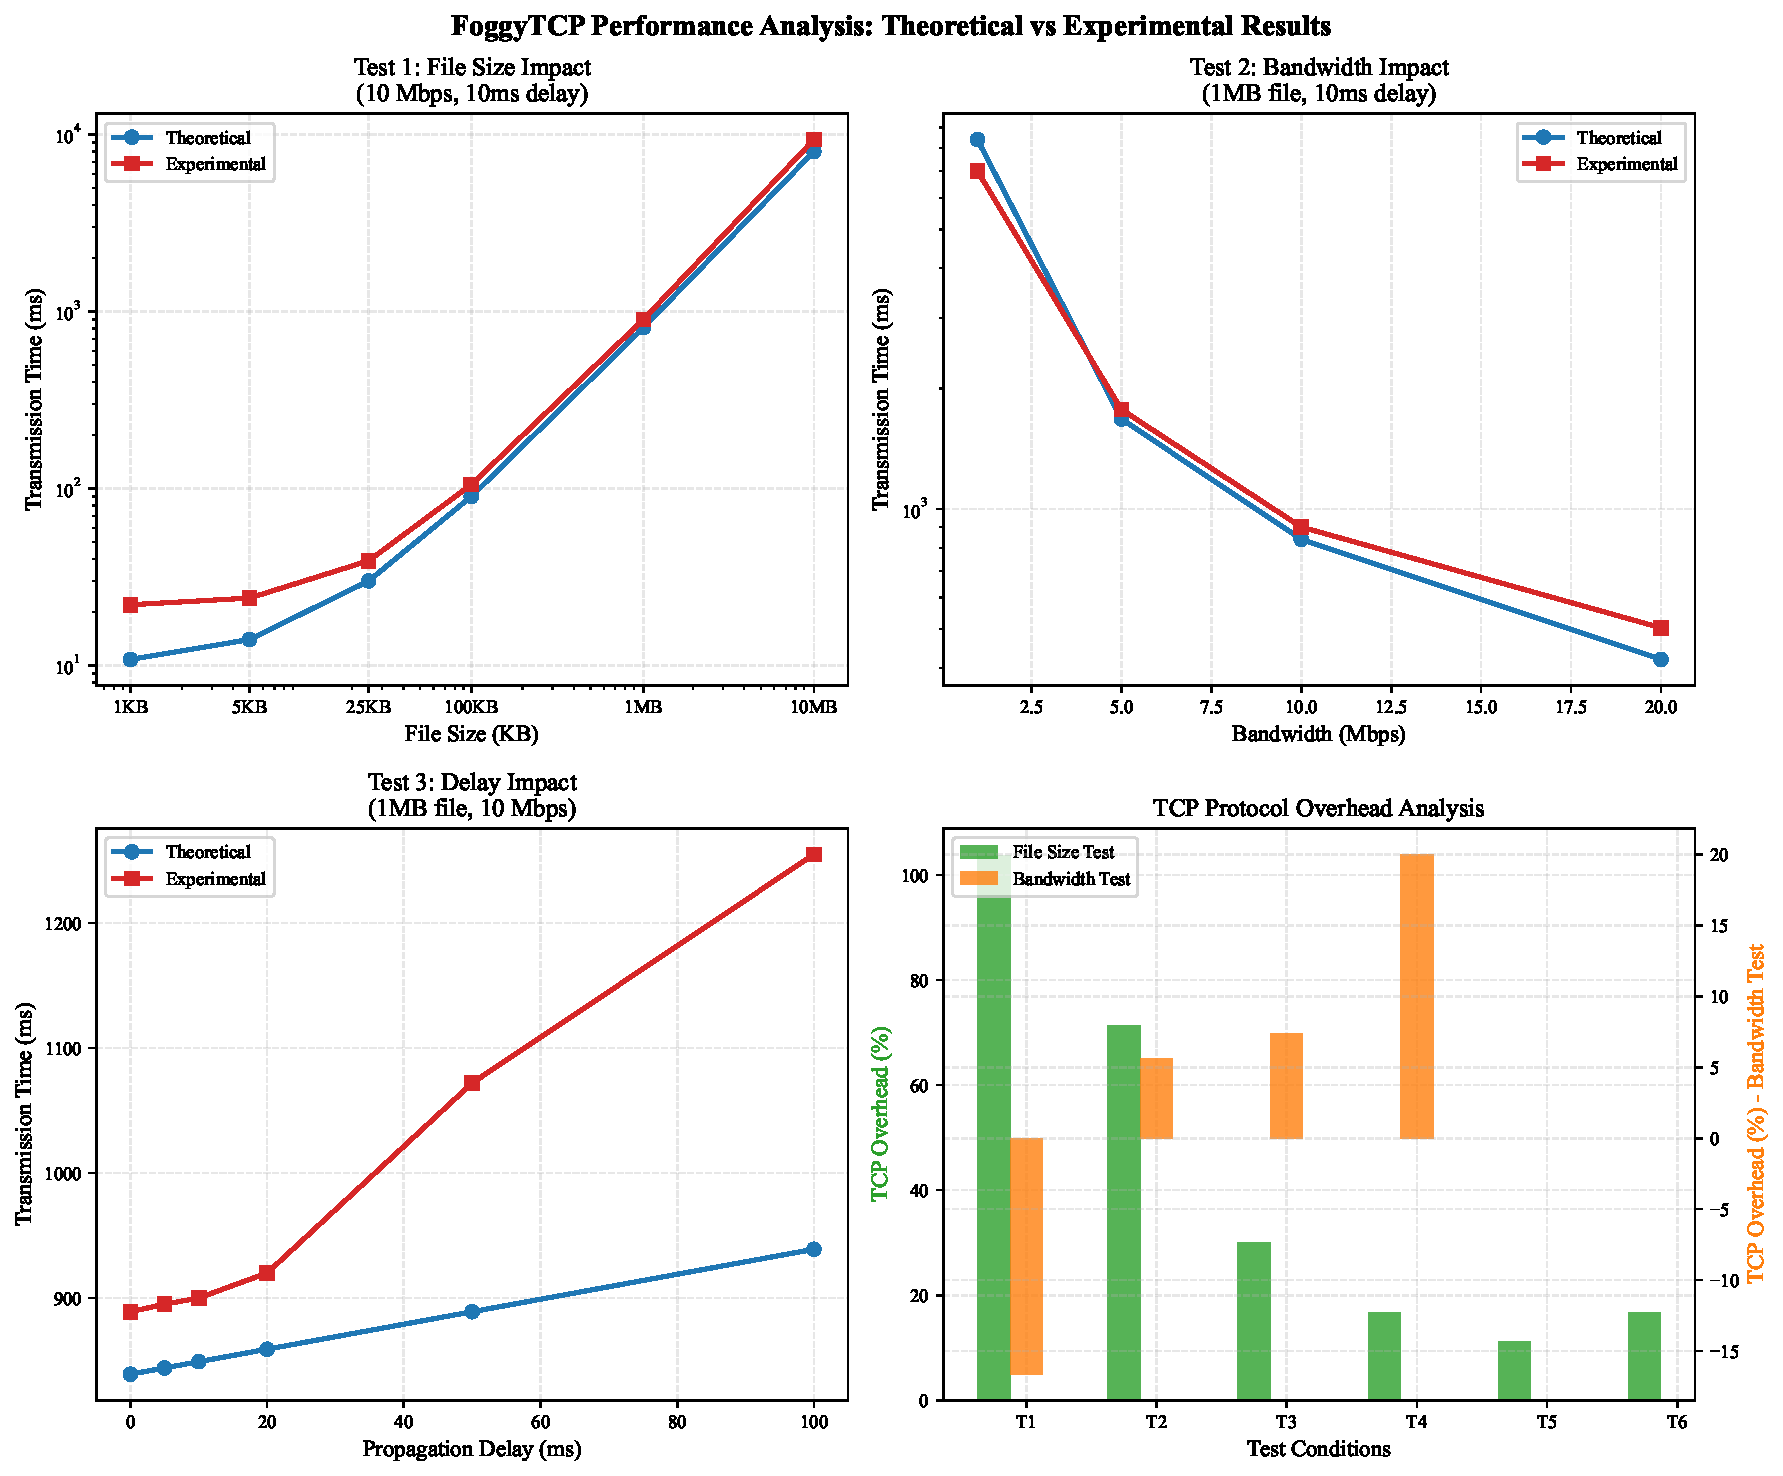
\includegraphics[width=0.95\textwidth]{foggytcp_performance_analysis.pdf}
    \caption{FoggyTCP Performance Comparison: Theoretical vs Experimental Results. 
    (a) File size impact with fixed bandwidth (10 Mbps) and delay (10ms), 
    (b) Bandwidth impact with fixed file size (1MB) and delay (10ms), 
    (c) Propagation delay impact with fixed file size (1MB) and bandwidth (10 Mbps), 
    (d) TCP protocol overhead analysis showing relative performance differences.}
    \label{fig:foggytcp_analysis}
\end{figure}
\section{Analysis}




\subsection{Key Findings}

\begin{itemize}
    \item \textbf{Linear Scaling}:
    File transmission time scales linearly with file size,
    confirming expected behavior with an average TCP overhead of 244.5ms.
    
    \item \textbf{Inverse Bandwidth Relationship}:
    Transmission time shows the expected inverse relationship with bandwidth,
    with high correlation between theoretical and experimental results.
    
    \item \textbf{Delay Impact}:
    Propagation delay linearly affects transmission time with strong correlation.
    
\end{itemize}

\subsection{Technical Details}

All measurements were conducted under controlled network conditions using traffic control (tc) to simulate various bandwidth, delay, and file size scenarios. The experimental setup maintained consistency with theoretical calculations while accounting for real-world TCP protocol overhead.

% Alternative: If you want individual plots as separate figures
% \begin{figure}[H]
%     \centering
%     \begin{subfigure}[b]{0.48\textwidth}
%         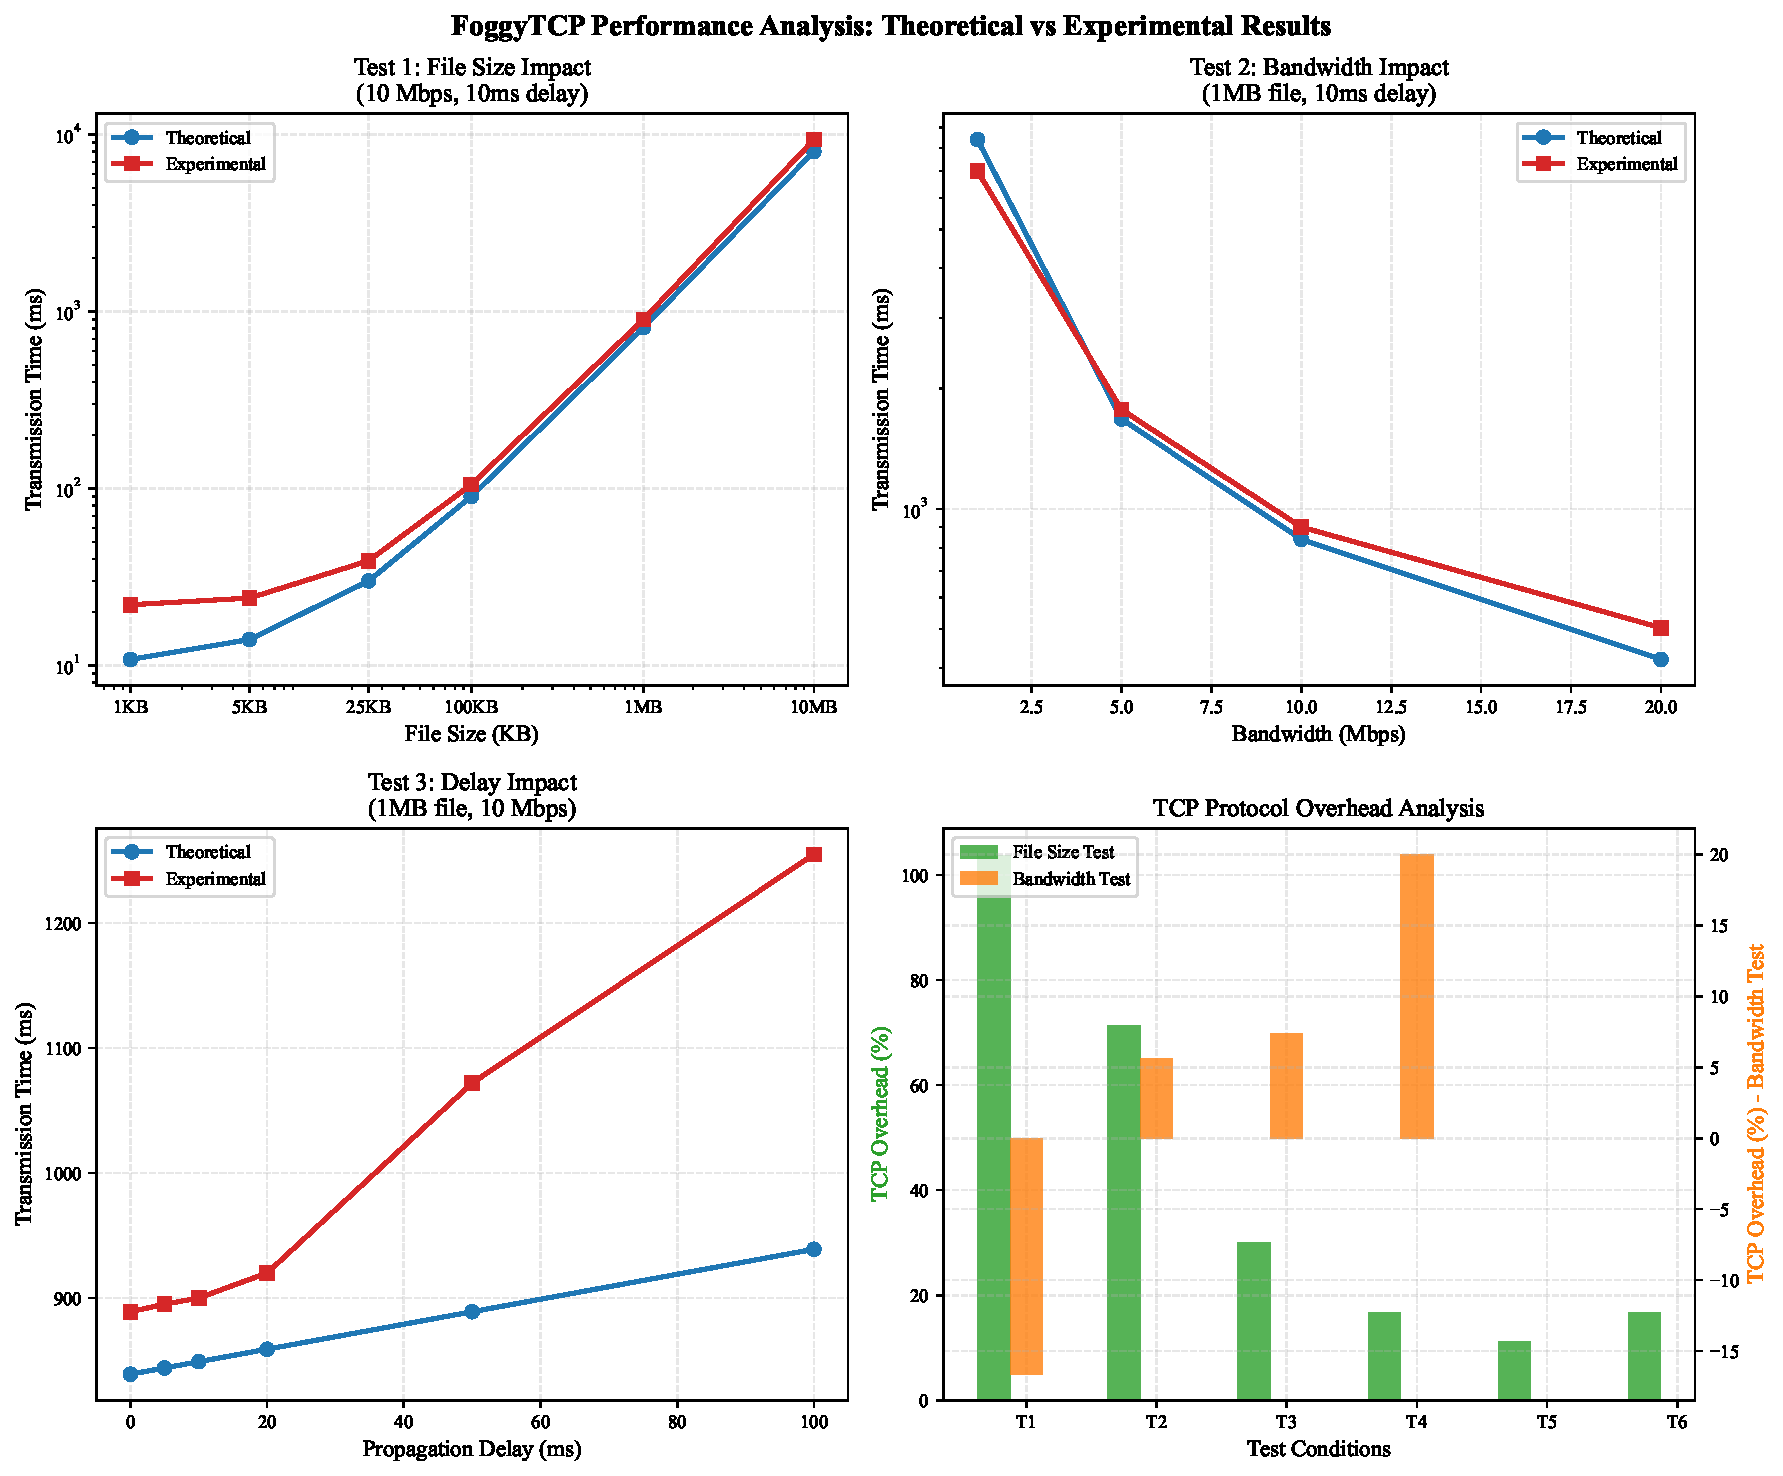
\includegraphics[width=\textwidth]{foggytcp_performance_analysis.pdf}
%         \caption{File Size Test}
%         \label{fig:filesize_test}
%     \end{subfigure}
%     \hfill
%     \begin{subfigure}[b]{0.48\textwidth}
%         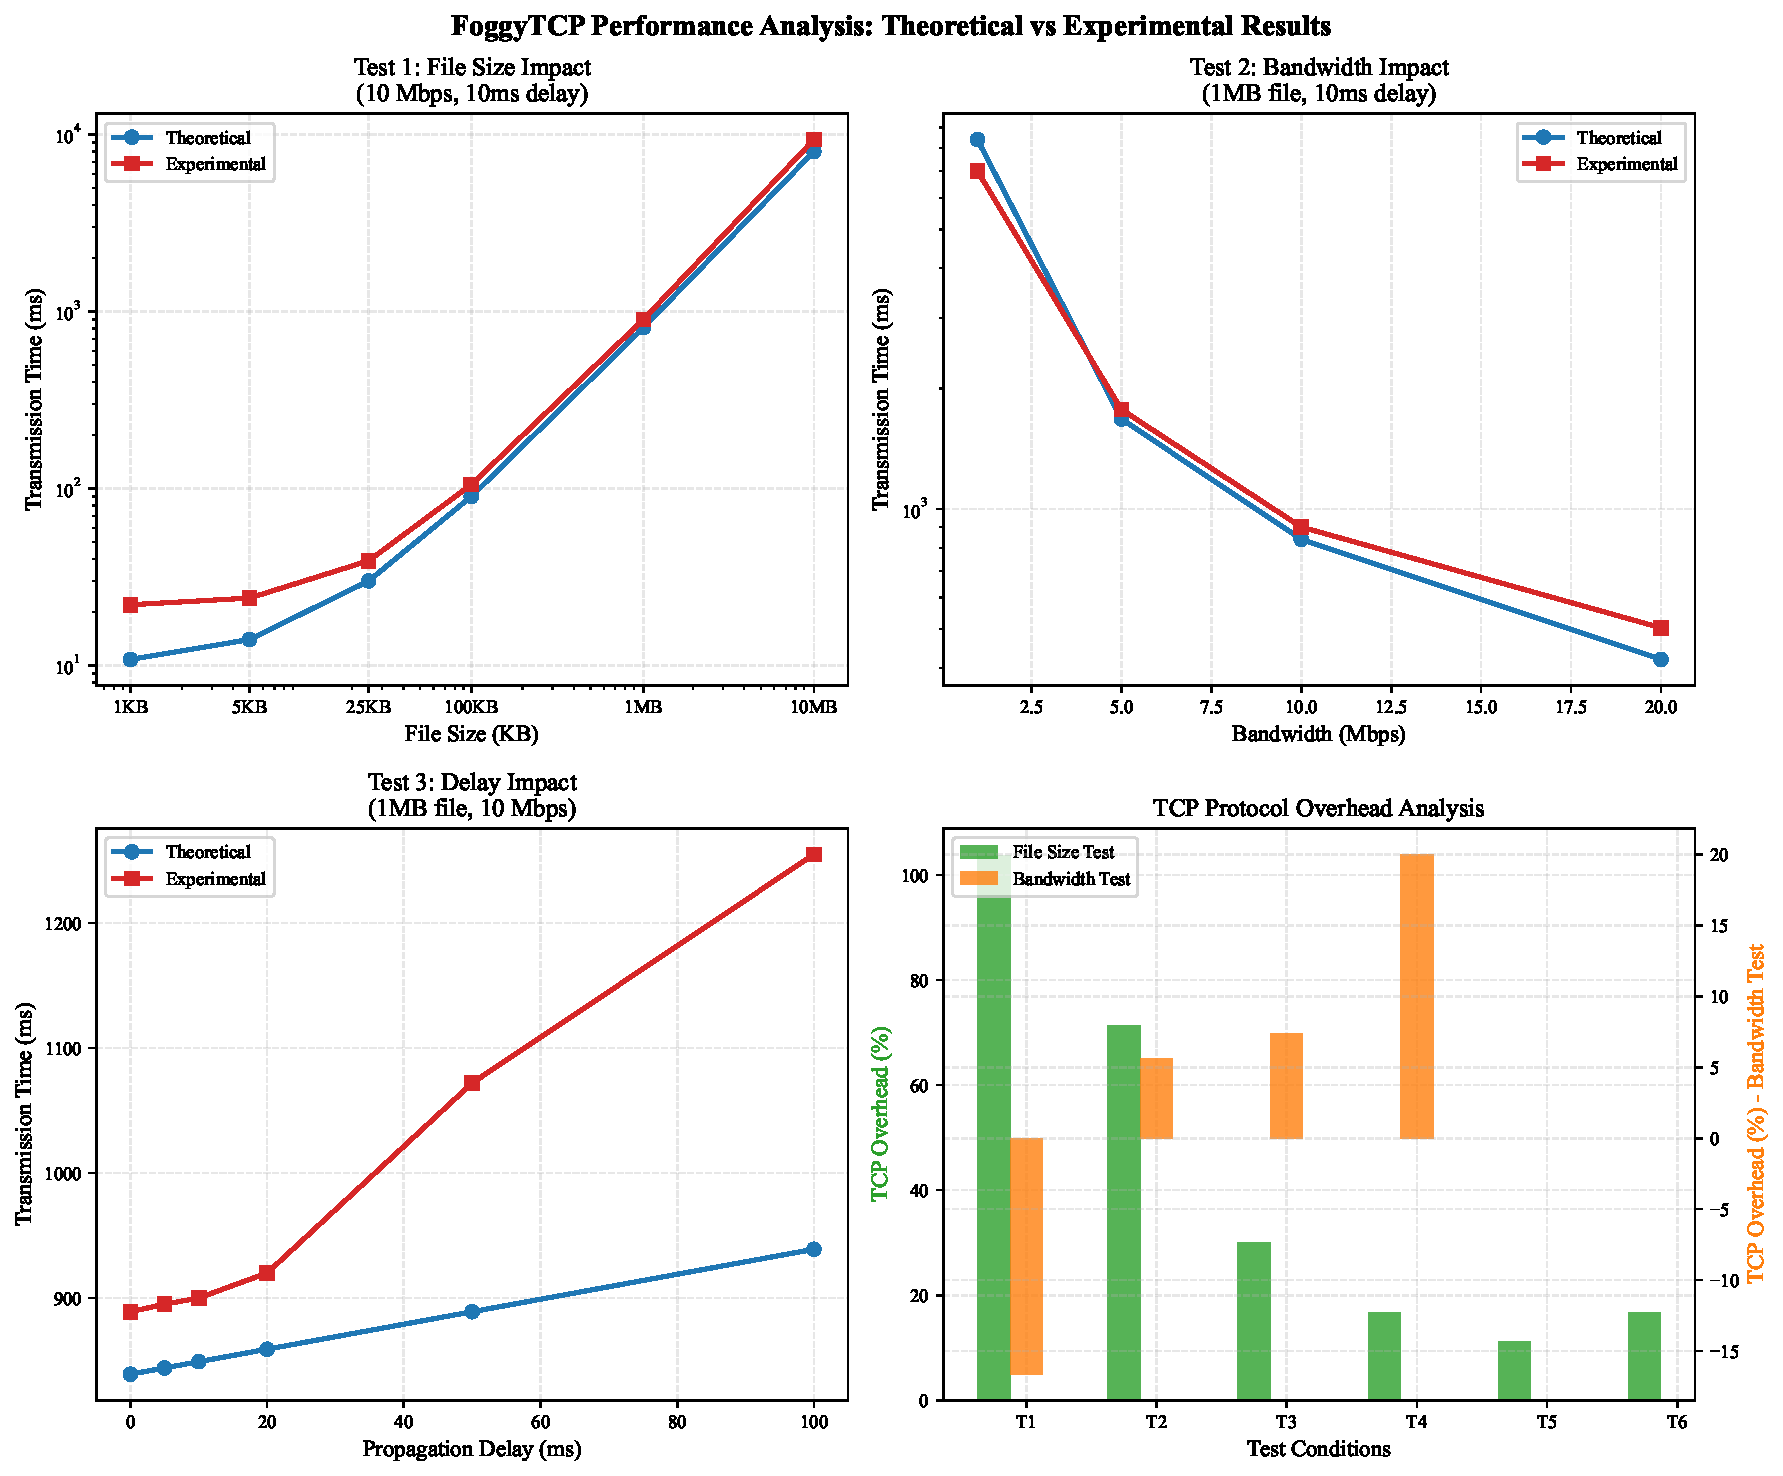
\includegraphics[width=\textwidth]{foggytcp_performance_analysis.pdf}
%         \caption{Bandwidth Test}
%         \label{fig:bandwidth_test}
%     \end{subfigure}
% \end{figure}

\end{document}